% Gibt die Klasse des Dokuments an
\documentclass[a4paper]{scrartcl}
% passende Kodierung für deutsche Sonderzeichen
%\usepackage[T1]{fontenc}
% bequemer Eingabezeichensatz(für Eszett etc.)
\usepackage[utf8]{inputenc}
% Für align-Umgebung etc.
\usepackage{amsmath, amsthm}
% For graphics
\usepackage[pdftex]{graphicx}


% deutsche Silbentrennung/Rechtschreibung
%\usepackage[ngerman]{babel}
\usepackage{amssymb}


% Eigene Befehle
\newtheorem{thm}{Theorem}[section]
\newtheorem{cor}[thm]{Korollar}
\newtheorem{defi}[thm]{Definition}
\newtheorem{lem}[thm]{Lemma}
\newtheorem{bem}[thm]{Bemerkung}

% Standardmengen
\newcommand{\R}{\mathbb{R}}
\newcommand{\Q}{\mathbb{Q}}
\newcommand{\Z}{\mathbb{Z}}
\newcommand{\N}{\mathbb{N}}
\newcommand{\E}{\mathbb{E}}
\newcommand{\rainf}{\rightarrow \infty}



\begin{document}
% Title
\title{Classification using Restricted Boltzmann Machines}
\author{Katarzyna Tarnowska \and Fritjof Wolf}
\maketitle
\newpage
% Abstract
\begin{abstract}
\textbf{Abstract:} 
\end{abstract}

% Textbody
\section{Introduction}
...
Hinton \cite{Hinton} describes three approaches to using Restricted Boltzmann Machines for classification task:
\begin{itemize}
    \item Using the hidden features learned by the RBM as the inputs for some standard discriminative method
    \item Training a separate RBM on each class
	\item Training a joint density model using a single RBM
\end{itemize}
The first method will not be discussed within this paper. Results from the second approach will be presented in the first section of this paper. The empirical results for the third approach will be described in the second section.
...
\subsection{Datasets}

\section{Empirical Results for Discriminative RBM}
This section describes the empirical results of a RBM trained with joint density model (the third approach of using RBM's for discrimination, described by Hinton \cite{Hinton}).
\subsection{Assumptions}
Joint density model assumes that RBM has two sets of visible units. Besides the units representing a data vector ({\bf x}), there are units representing a label (as a binary vector) - {\bf y}. As a result, there are also two sets of weights: between data and hidden units ({\bf W}) and between label units and hidden units ({\bf U}). 
\begin{center}
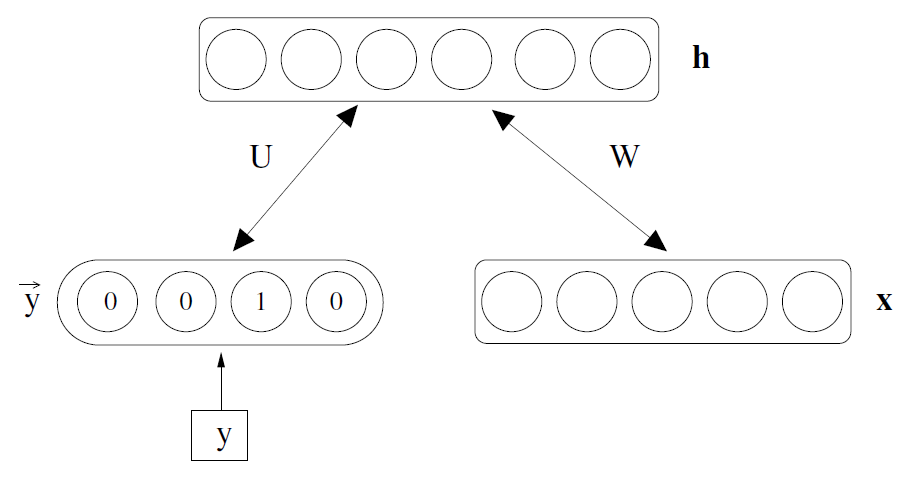
\includegraphics[width=6cm]{images/jointProbModel.png}
\captionof{figure}{Joint probability model of Restricted Boltzmann Machines}  
\end{center}
Model learns joint probability distribution with n-step contrastive divergence (CD) algorithm.
\begin{center}
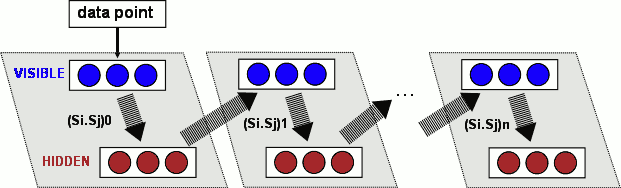
\includegraphics[width=14cm]{images/trainRBM.png}
\captionof{figure}{Illustration of N-step Contrastive Divergence algorithm}  
\end{center} 
\par Class prediction is performed by done by choosing the most likely label given the input, under the learned model. In more detail, by fixing the visible units corresponding to the test data input and sampling target units, with the use of learned weights. In the last sampling iteration the target units are set to probabilities values instead of stochastic binary units. The predicted class is the position in the binary vector with the highest probability.
\par Training is performed on mini-batches of the training set. In terms of the CD algorithm, it means that weights are updated after estimating a gradient on a subset of training cases (a "mini-batch"), instead of on a one single training case. Such approach is known to be more efficient, because of possible use of CPU parallelism and multi-threading.
\par Tests were carried out on MNIST dataset, divided into training and test-sets. The data was binarized (with the binarization threshold of 0.5). 

\subsection{Results}
The aim of testing implemented RBM was finding optimal hyperparameters (optimal model parameters) and calculate classification metrics. The most important metric for classification task is accuracy, that is, the percentage of right predictions. Accuracy was computed by comparing the label predicted by RBM classifier with the original label. Wrong predictions were counted.
\par The results from training an RBM with different learning rates are shown on the figure below.
\begin{center}
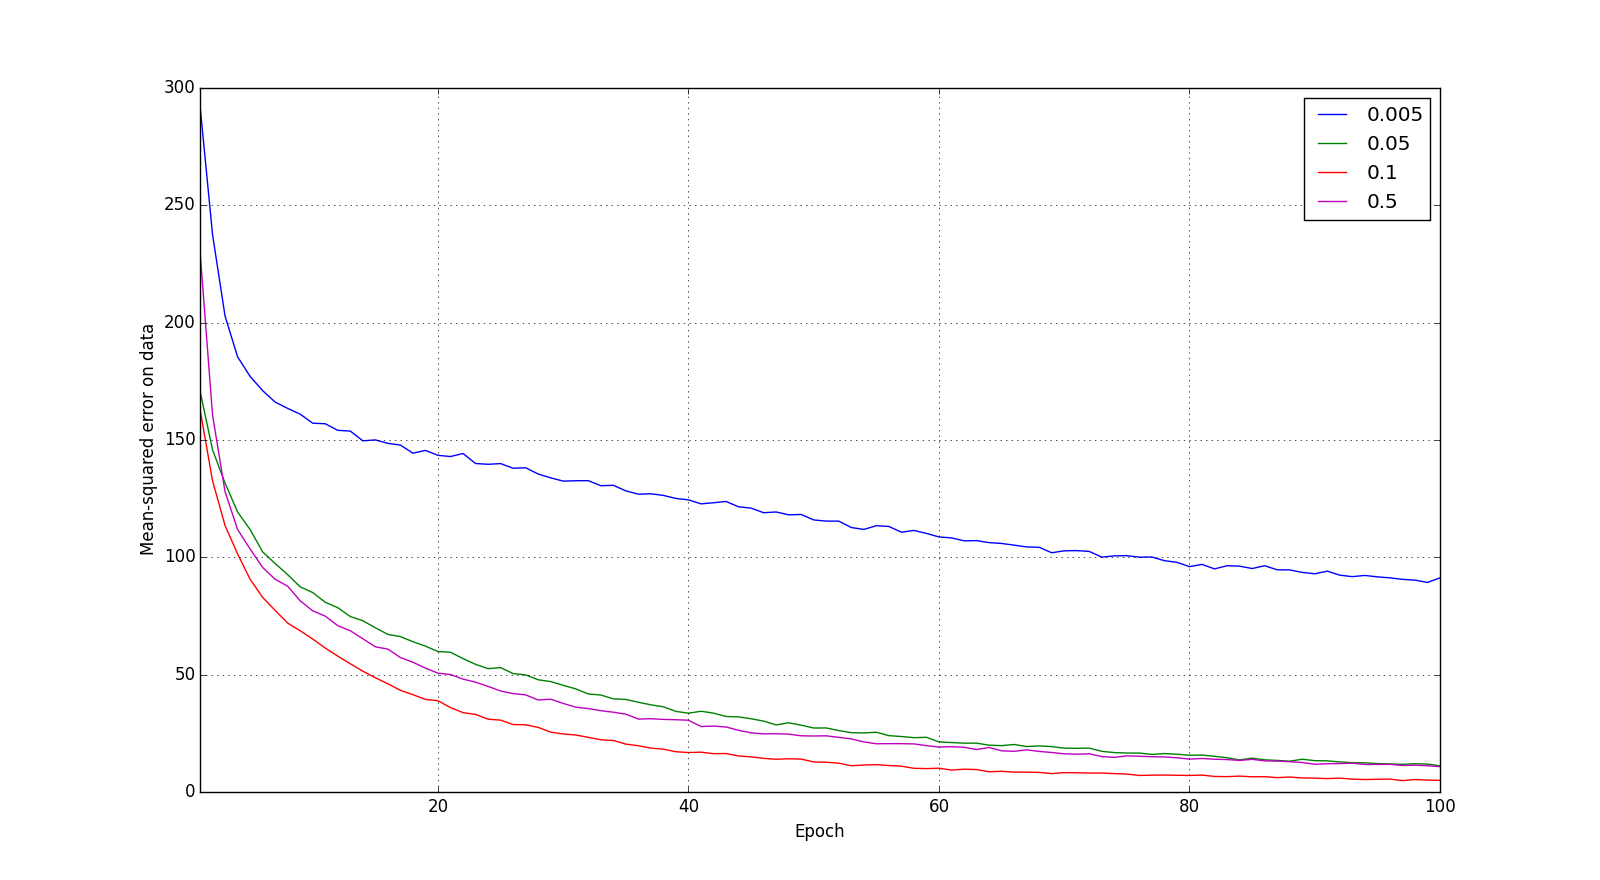
\includegraphics[width=16cm]{images/lr.png}
\captionof{figure}{Covergence comparison for different learning rates}  
\end{center}
Learning rate of a magnitude between $10^{-2}$ and $10^{-3}$ seems to be optimal. The exact optimal magnitude depends also on the training size, as tests on larger data sizes have shown (for example for smaller data sizes 0.1 was optimal, while for original sizes of 60000 - 0.01 was optimal).
\par The second test was done on number of hidden units. As figure below shows, the higher the number of hidden units, the better convergence of reconstruction error. On the other hand, greater hidden layer size causes longer training time.
\begin{center}
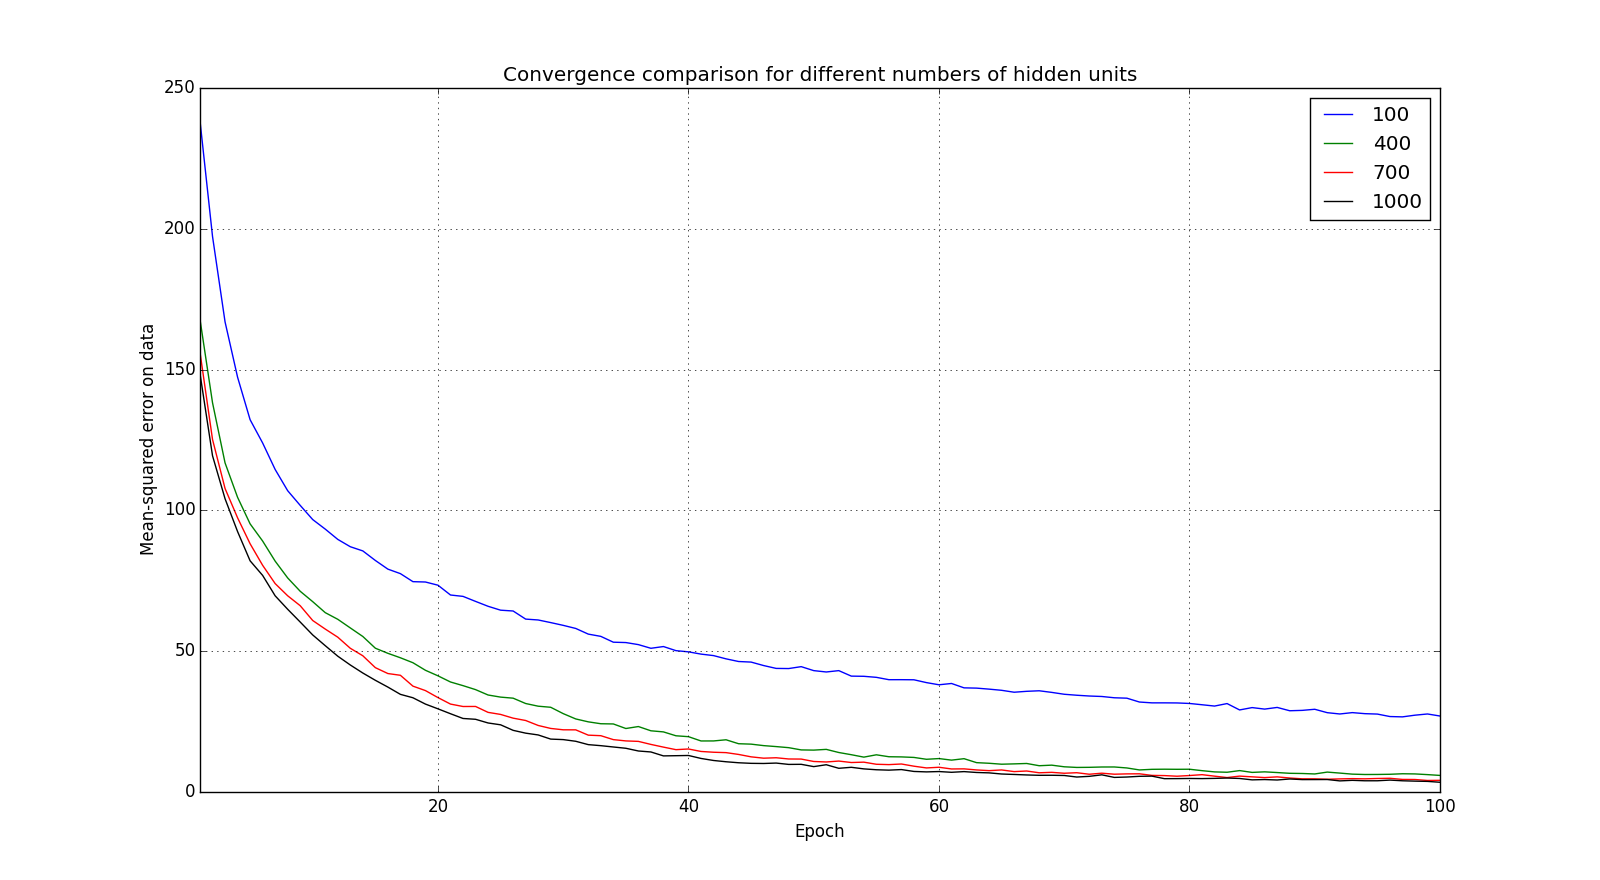
\includegraphics[width=16cm]{images/hu.png}
\captionof{figure}{Covergence comparison for different number of hidden units}  
\end{center}
\par number of steps for contrastive divergence algorithm.
\par Experiments with momentum
\par Original data and reconstructions with optimal hyperparameters
% Literature
\begin{thebibliography}{9}
   \bibitem[1]{Hopfield} Hopfield, J.J. (1984) \emph{Neurons with graded response have collective computational properties like those of two-state neurons} (Proc. Natl. Acad. Sci. USA)
   \bibitem[2]{Hinton} Hinton, G. (2010) \emph{A Pratical Guide to Training Restricted Boltzmann Machines.} (UTML TR 2010-003)
   
\end{thebibliography}
\end{document}